\documentclass[12pt]{article}

\usepackage{amsmath,amssymb}
\usepackage{graphicx}
\usepackage{float}
\usepackage[colorlinks=true, linkcolor=blue]{hyperref} 

\usepackage{xepersian}

\settextfont[
Path = fonts/ ,
Extension = .ttf ,
Scale = 1.1
]{Yas}

\setdigitfont[
Path = fonts/ ,
Extension = .ttf ,
Scale = 1.1
]{Yas}

\linespread{1.15}

\begin{document}
	
	\section{درونیابی لاگرانژ و اسپلاین مکعبی طبیعی}
	
	\subsection{صورت مسئله}
	
	در این تمرین، مجموعهٔ نقاط زیر در نظر گرفته شده است:
	\[
	(1,1),\ (2,3),\ (3,5),\ (4,8),\ (5,5),\ (6,2).
	\]
	
	هدف، به‌دست آوردن چندجمله‌ای درونیاب لاگرانژ برای این نقاط و همچنین محاسبهٔ اسپلاین مکعبی طبیعی روی بازه‌های متوالی آن‌ها است. در روش لاگرانژ، یک چندجمله‌ای واحد از تمام نقاط عبور می‌کند؛ اما در روش اسپلاین، برای هر بازه یک چندجمله‌ای جداگانه ساخته می‌شود و این چندجمله‌ای‌ها در نقاط اتصال، شرایط همواری لازم را دارند.
	
	\subsection{درونیابی لاگرانژ}
	
	درونیابی لاگرانژ روشی برای ساختن چندجمله‌ای‌ای است که از تمام نقاط داده‌شده عبور کند. اگر نقاط داده‌شده به‌صورت زیر باشند:
	\[
	(x_0,y_0),\ (x_1,y_1),\ \ldots,\ (x_n,y_n),
	\]
	چندجمله‌ای درونیاب لاگرانژ به‌صورت رابطه~\eqref{eq:lagrange-poly} تعریف می‌شود.
	\begin{equation}
		P(x)=\sum_{i=0}^{n} y_i L_i(x)
		\label{eq:lagrange-poly}
	\end{equation}
	
	در این رابطه، $L_i(x)$ پایهٔ لاگرانژ متناظر با نقطهٔ $i$ام است و از رابطه~\eqref{eq:lagrange-basis} به‌دست می‌آید.
	\begin{equation}
		L_i(x)=
		\prod_{\substack{j=0 \\ j\neq i}}^{n}
		\frac{x-x_j}{x_i-x_j}.
		\label{eq:lagrange-basis}
	\end{equation}
	
	پایهٔ لاگرانژ به‌گونه‌ای ساخته می‌شود که در نقطهٔ $x_i$ مقدار آن برابر $1$ و در سایر نقاط داده‌شده مقدار آن برابر صفر باشد. بنابراین در رابطه~\eqref{eq:lagrange-poly}، هر جمله فقط مقدار تابع در نقطهٔ مربوط به خود را در چندجمله‌ای نهایی اثر می‌دهد.
	
	با جایگذاری نقاط داده‌شده در رابطه‌های~\eqref{eq:lagrange-poly} و~\eqref{eq:lagrange-basis}، چندجمله‌ای نهایی لاگرانژ به‌صورت رابطه~\eqref{eq:lagrange-result} به‌دست می‌آید.
	\begin{equation}
		P(x)=
		\frac{7x^5}{40}
		-\frac{71x^4}{24}
		+\frac{147x^3}{8}
		-\frac{1249x^2}{24}
		+\frac{1369x}{20}
		-31
		\label{eq:lagrange-result}
	\end{equation}
	
	این چندجمله‌ای از همهٔ نقاط مسئله عبور می‌کند. برای نمونه داریم:
	\[
	P(1)=1,\quad
	P(2)=3,\quad
	P(3)=5,\quad
	P(4)=8,\quad
	P(5)=5,\quad
	P(6)=2.
	\]
	
	\subsubsection{برنامهٔ محاسبهٔ درونیابی لاگرانژ}
	
	در \figurename~\ref{fig:lagrange-code}، کد مربوط به محاسبهٔ چندجمله‌ای درونیاب لاگرانژ نمایش داده شده است.
	
	\begin{figure}[H]
		\centering
		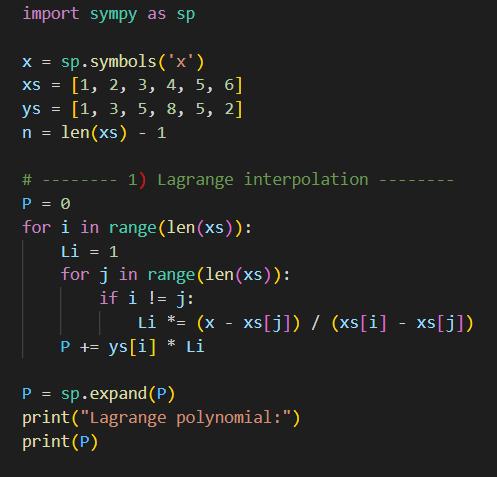
\includegraphics[width=0.95\textwidth, height=11cm, keepaspectratio]{lagrange-code.png}
		\caption{کد محاسبهٔ درونیابی لاگرانژ}
		\label{fig:lagrange-code}
	\end{figure}
	
	در این کد، ابتدا داده‌های ورودی در دو فهرست $xs$ و $ys$ ذخیره شده‌اند. سپس برای هر نقطه، پایهٔ لاگرانژ مطابق رابطه~\eqref{eq:lagrange-basis} ساخته شده و در مقدار تابع در همان نقطه ضرب شده است. در پایان، مجموع جمله‌ها طبق رابطه~\eqref{eq:lagrange-poly} محاسبه، ساده و بسط داده شده است. محاسبات نمادین این بخش با استفاده از یک کتابخانهٔ پایتونی انجام شده است.\footnote{SymPy}
	
	در \figurename~\ref{fig:lagrange-result}، خروجی اجرای برنامه نمایش داده شده است.
	
	\begin{figure}[H]
		\centering
		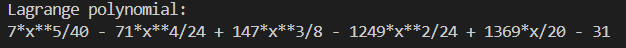
\includegraphics[width=0.95\textwidth]{lagrange-result.png}
		\caption{خروجی محاسبهٔ چندجمله‌ای لاگرانژ}
		\label{fig:lagrange-result}
	\end{figure}
	
	همان‌طور که در \figurename~\ref{fig:lagrange-result} دیده می‌شود، برنامه پس از تشکیل پایه‌های لاگرانژ، چندجمله‌ای نهایی را ساده کرده و عبارت نوشته‌شده در رابطه~\eqref{eq:lagrange-result} را به‌دست می‌دهد.
	
	\subsection{اسپلاین مکعبی طبیعی}
	
	در روش اسپلاین مکعبی، به‌جای ساختن یک چندجمله‌ای واحد برای تمام نقاط، برای هر بازهٔ بین دو نقطهٔ متوالی یک چندجمله‌ای درجهٔ سه ساخته می‌شود. در این مسئله $6$ نقطه وجود دارد؛ بنابراین $5$ بازه و در نتیجه $5$ چندجمله‌ای مکعبی خواهیم داشت.
	
	فرم کلی هر قطعه از اسپلاین به‌صورت رابطه~\eqref{eq:spline-form} در نظر گرفته می‌شود.
	\begin{equation}
		S_i(x)=a_i x^3+b_i x^2+c_i x+d_i.
		\label{eq:spline-form}
	\end{equation}
	
	برای تعیین ضرایب مجهول، چند شرط روی قطعه‌های اسپلاین اعمال می‌شود. نخست، هر قطعه باید از دو سر بازهٔ خود عبور کند. همچنین در نقاط اتصال، مقدار تابع، مشتق اول و مشتق دوم باید پیوسته باشند. افزون بر این، چون اسپلاین از نوع طبیعی است، مشتق دوم در دو سر کل بازه برابر صفر قرار داده می‌شود.
	
	شرط طبیعی بودن اسپلاین در این مسئله به‌صورت رابطه~\eqref{eq:natural-condition} نوشته می‌شود.
	\begin{equation}
		S''(1)=0,\qquad S''(6)=0.
		\label{eq:natural-condition}
	\end{equation}
	
	با اعمال این شرط‌ها، یک دستگاه معادلات برای ضرایب مجهول تشکیل می‌شود. حل این دستگاه، قطعه‌های زیر را برای اسپلاین مکعبی طبیعی به‌دست می‌دهد:
	
	\begin{align}
		S_0(x) &=
		-\frac{39x^3}{209}
		+\frac{117x^2}{209}
		+\frac{340x}{209}
		-1,
		\qquad 1 \leq x \leq 2,
		\label{eq:s0}
		\\[4pt]
		S_1(x) &=
		\frac{195x^3}{209}
		-\frac{117x^2}{19}
		+\frac{3148x}{209}
		-\frac{2081}{209},
		\qquad 2 \leq x \leq 3,
		\label{eq:s1}
		\\[4pt]
		S_2(x) &=
		-\frac{28x^3}{11}
		+\frac{5256x^2}{209}
		-\frac{16481x}{209}
		+\frac{17548}{209},
		\qquad 3 \leq x \leq 4,
		\label{eq:s2}
		\\[4pt]
		S_3(x) &=
		\frac{470x^3}{209}
		-\frac{6768x^2}{209}
		+\frac{31615x}{209}
		-\frac{46580}{209},
		\qquad 4 \leq x \leq 5,
		\label{eq:s3}
		\\[4pt]
		S_4(x) &=
		-\frac{94x^3}{209}
		+\frac{1692x^2}{209}
		-\frac{10685x}{209}
		+\frac{23920}{209},
		\qquad 5 \leq x \leq 6.
		\label{eq:s4}
	\end{align}
	
	بنابراین تابع اسپلاین به‌صورت تکه‌ای رابطه~\eqref{eq:spline-piecewise} تعریف می‌شود.
	\begin{equation}
		S(x)=
		\begin{cases}
			S_0(x), & 1 \leq x \leq 2,\\
			S_1(x), & 2 \leq x \leq 3,\\
			S_2(x), & 3 \leq x \leq 4,\\
			S_3(x), & 4 \leq x \leq 5,\\
			S_4(x), & 5 \leq x \leq 6.
		\end{cases}
		\label{eq:spline-piecewise}
	\end{equation}
	
	رابطه~\eqref{eq:spline-piecewise} نشان می‌دهد که برخلاف روش لاگرانژ، در اینجا یک تابع تکه‌ای ساخته شده است. هر قطعه فقط روی بازهٔ خودش معتبر است، اما همهٔ قطعه‌ها در نقاط اتصال به‌صورت هموار به یکدیگر وصل می‌شوند.
	
	\subsubsection{برنامهٔ محاسبهٔ اسپلاین مکعبی طبیعی}
	
	در \figurename~\ref{fig:spline-code}، کد مربوط به محاسبهٔ اسپلاین مکعبی طبیعی نمایش داده شده است.
	
	\begin{figure}[H]
		\centering
		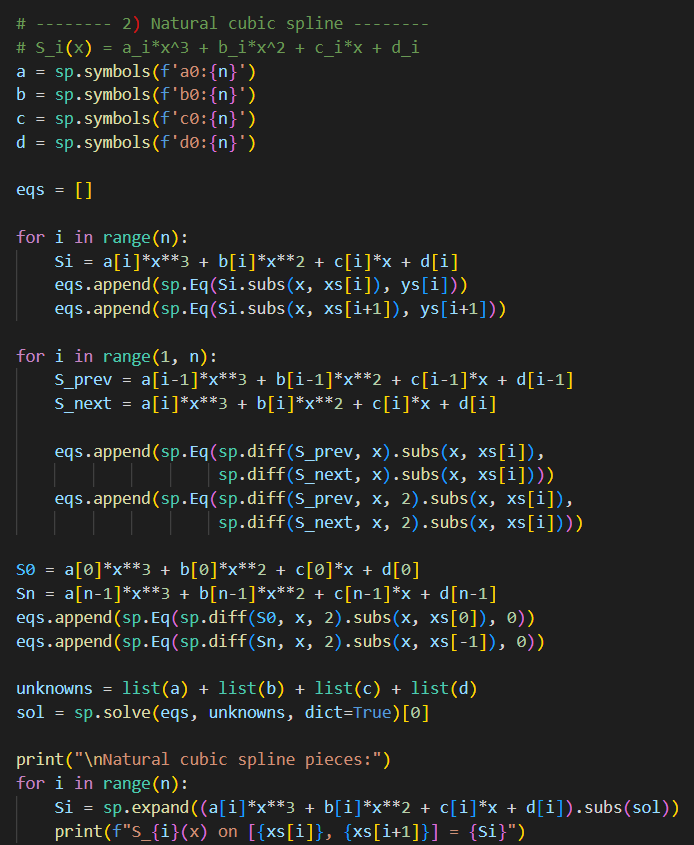
\includegraphics[width=0.95\textwidth]{spline-code.png}
		\caption{کد محاسبهٔ اسپلاین مکعبی طبیعی}
		\label{fig:spline-code}
	\end{figure}
	
	در این کد، برای هر بازه یک چندجمله‌ای مکعبی مطابق فرم کلی رابطه~\eqref{eq:spline-form} تعریف شده است. سپس شرط عبور هر قطعه از دو سر بازهٔ خودش نوشته شده است. برای نقاط داخلی نیز پیوستگی مقدار تابع، مشتق اول و مشتق دوم اعمال شده است. در پایان، شرط طبیعی بودن اسپلاین مطابق رابطه~\eqref{eq:natural-condition} به دستگاه معادلات افزوده شده و دستگاه حاصل حل شده است.
	
	در \figurename~\ref{fig:spline-result}، خروجی اجرای برنامه نمایش داده شده است.
	
	\begin{figure}[H]
		\centering
		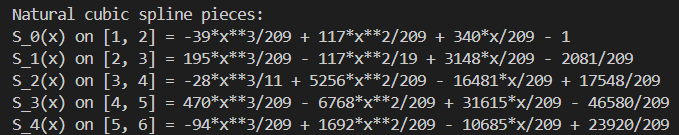
\includegraphics[width=0.95\textwidth]{spline-result.png}
		\caption{خروجی محاسبهٔ اسپلاین مکعبی طبیعی}
		\label{fig:spline-result}
	\end{figure}
	
	خروجی \figurename~\ref{fig:spline-result} شامل ضرایب قطعه‌های مختلف اسپلاین است. این ضرایب همان قطعه‌هایی را می‌سازند که در رابطه‌های~\eqref{eq:s0} تا~\eqref{eq:s4} نوشته شده‌اند.
	
	\subsection{جمع‌بندی}
	
	در این تمرین، دو روش درونیابی برای مجموعهٔ داده‌های مسئله بررسی شدند. روش لاگرانژ یک چندجمله‌ای واحد تولید کرد که از تمام نقاط داده‌شده عبور می‌کند. نتیجهٔ این روش در رابطه~\eqref{eq:lagrange-result} نوشته شد.
	
	در مقابل، روش اسپلاین مکعبی طبیعی یک تابع تکه‌ای ساخت که هر قطعهٔ آن روی یک بازهٔ مشخص تعریف می‌شود. این تابع علاوه بر عبور از نقاط داده‌شده، در نقاط اتصال نیز پیوستگی مقدار تابع، مشتق اول و مشتق دوم را حفظ می‌کند. همچنین با اعمال شرط طبیعی بودن، مشتق دوم در دو سر بازهٔ اصلی برابر صفر قرار گرفت.
	\section{تحلیل زمان اجرای الگوریتم‌ها و مصورسازی داده‌ها}
	
	\subsection{صورت مسئله}
	در این بخش از پروژه، فایل داده‌ای با فرمت اکسل شامل زمان اجرای سه الگوریتم مختلف به ازای داده‌های ورودی با اندازه‌های متفاوت ($100$ تا $600$ کیلوبایت) مورد بررسی قرار گرفته است. هدف، خواندن این فایل به صورت پویا با استفاده از زبان پایتون، رسم سه نوع نمودار (خطی، میله‌ای و جعبه‌ای)، محاسبه میانگین زمان اجرا برای یک الگوریتم خاص، و در نهایت بررسی قابلیت انعطاف‌پذیری کد در صورت افزوده شدن داده‌های جدید به فایل اکسل است.
	
	\subsection{خواندن فایل و رسم نمودارها (بدون داده $700$ کیلوبایت)}
	برای حل این بخش، از کتابخانه‌های پانداس\footnote{\lr{pandas}} جهت خواندن و پردازش داده‌ها و از مت‌پلات‌لیب\footnote{\lr{matplotlib}} جهت رسم نمودارها استفاده شده است. کد به گونه‌ای نوشته شده است که نام ستون‌ها و مقادیر آن‌ها را به صورت پویا پردازش کرده و عبارات اضافی مانند کیلوبایت\footnote{\lr{KB}} را حذف می‌کند تا داده‌ها به اعداد قابل محاسبه تبدیل شوند.
	
	در \figurename~\ref{fig:plot-code}، بخش مربوط به پردازش داده‌ها و کدهای رسم نمودارها در پایتون آورده شده است.
	
	\begin{figure}[H]
		\centering
		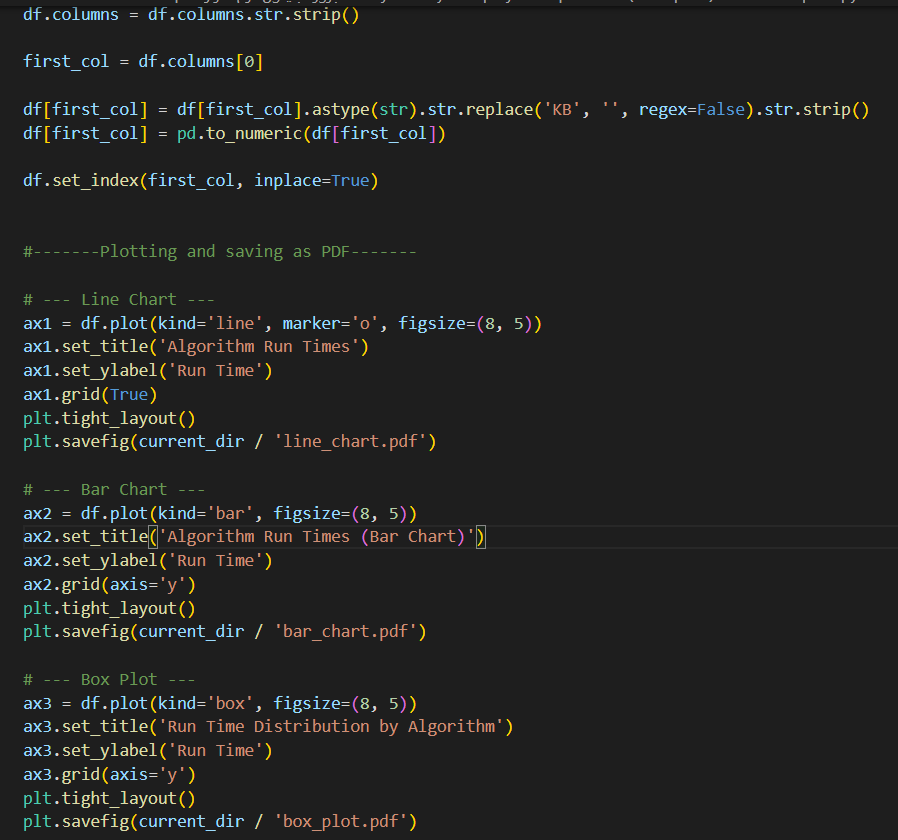
\includegraphics[width=0.95\textwidth, height=11cm, keepaspectratio]{plot_code.png} 
		\caption{کد پایتون برای پردازش داده‌های اکسل و رسم نمودارها}
		\label{fig:plot-code}
	\end{figure}
	
	پس از اجرای کد بر روی داده‌های اولیه ($100$ تا $600$ کیلوبایت)، سه نمودار زیر حاصل می‌شود.
	
	\subsubsection[تحلیل نمودار خطی]{تحلیل نمودار خطی\footnote{\lr{Line Chart}}}
	در \figurename~\ref{fig:line-before} نمودار خطی زمان اجرای الگوریتم‌ها رسم شده است.
	
	\begin{figure}[H]
		\centering
		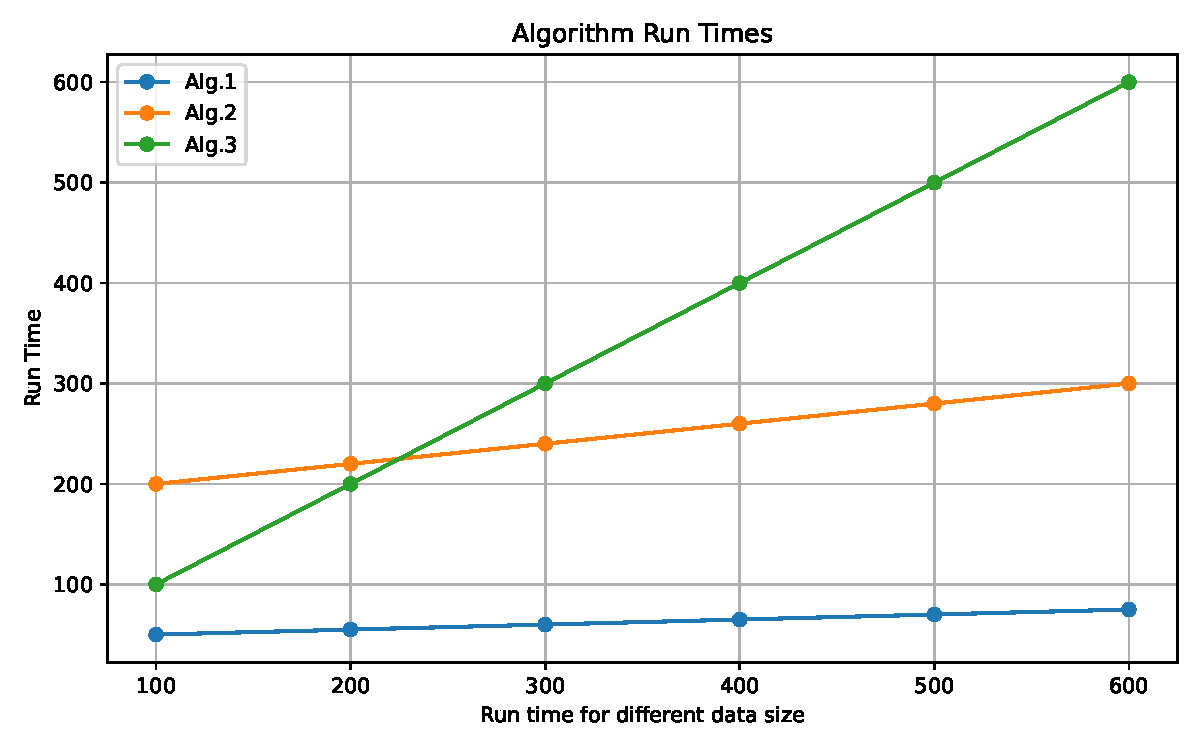
\includegraphics[width=0.8\textwidth]{line_before.pdf} 
		\caption{نمودار خطی زمان اجرای الگوریتم‌ها ($100$ تا $600$ کیلوبایت)}
		\label{fig:line-before}
	\end{figure}
	\textbf{تحلیل:} همان‌طور که از نمودار خطی پیداست، زمان اجرای الگوریتم $3$\footnote{\lr{Alg.3}} با افزایش حجم داده‌ها با شیب تندی افزایش می‌یابد (از $100$ به $600$) که نشان‌دهنده حساسیت بالای این الگوریتم به حجم داده است. در مقابل، الگوریتم $1$\footnote{\lr{Alg.1}} کمترین شیب و رشد را داشته و عملکرد بسیار پایداری دارد. الگوریتم $2$\footnote{\lr{Alg.2}} با وجود اینکه در داده‌های کم ($100$ کیلوبایت) بیشترین زمان اجرا را دارد، اما رشد آن ملایم‌تر از الگوریتم $3$ است و در حجم‌های بالاتر، از آن جا می‌ماند.
	
	\subsubsection[تحلیل نمودار میله‌ای]{تحلیل نمودار میله‌ای\footnote{\lr{Bar Chart}}}
	در \figurename~\ref{fig:bar-before} نمودار میله‌ای داده‌ها قابل مشاهده است.
	
	\begin{figure}[H]
		\centering
		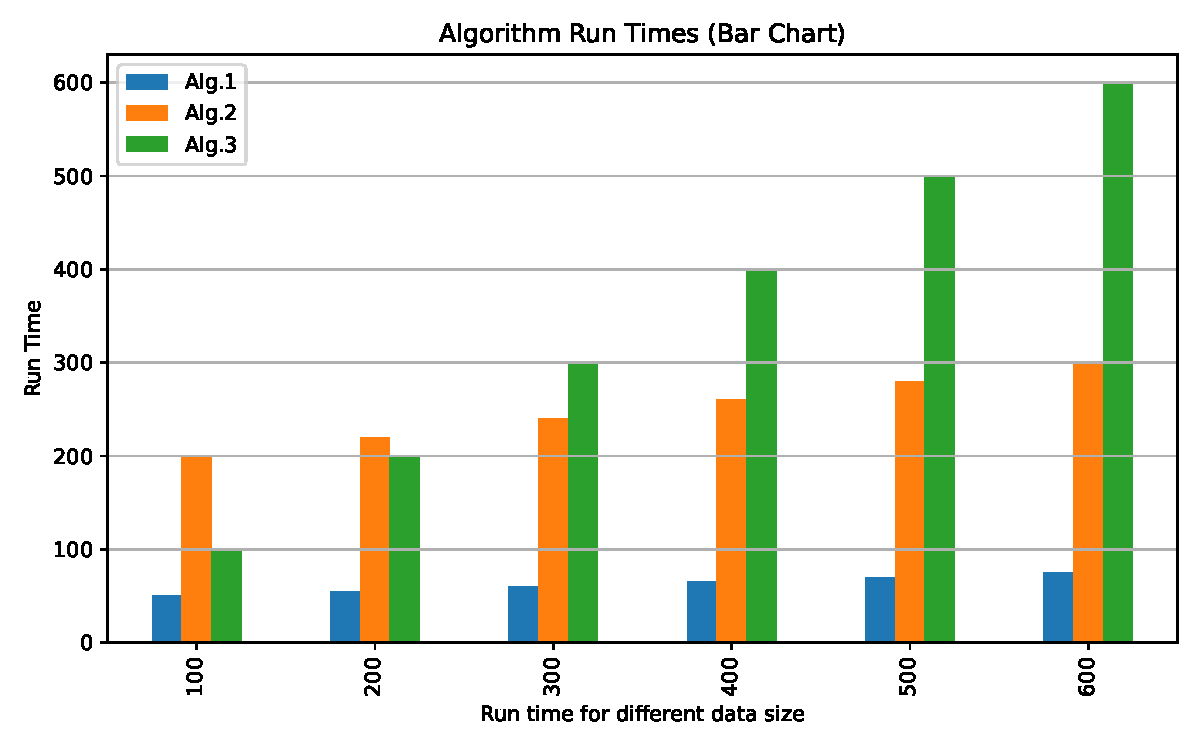
\includegraphics[width=0.8\textwidth]{bar_before.pdf} 
		\caption{نمودار میله‌ای مقایسه زمان اجرای الگوریتم‌ها در حجم داده‌های مختلف}
		\label{fig:bar-before}
	\end{figure}
	\textbf{تحلیل:} نمودار میله‌ای به خوبی امکان مقایسه نظیر‌به‌نظیر الگوریتم‌ها را در هر حجم داده فراهم می‌کند. کاملاً مشخص است که در حجم $600$ کیلوبایت، میله مربوط به الگوریتم $3$ بلندترین ارتفاع را دارد، در حالی که الگوریتم $1$ با زمان اجرای $75$، با اختلاف بسیار چشمگیری سریع‌تر از دو الگوریتم دیگر عمل کرده است.
	
	\subsubsection[تحلیل نمودار جعبه‌ای]{تحلیل نمودار جعبه‌ای\footnote{\lr{Box Plot}}}
	در \figurename~\ref{fig:box-before} نمودار جعبه‌ای برای بررسی توزیع داده‌ها رسم شده است.
	
	\begin{figure}[H]
		\centering
		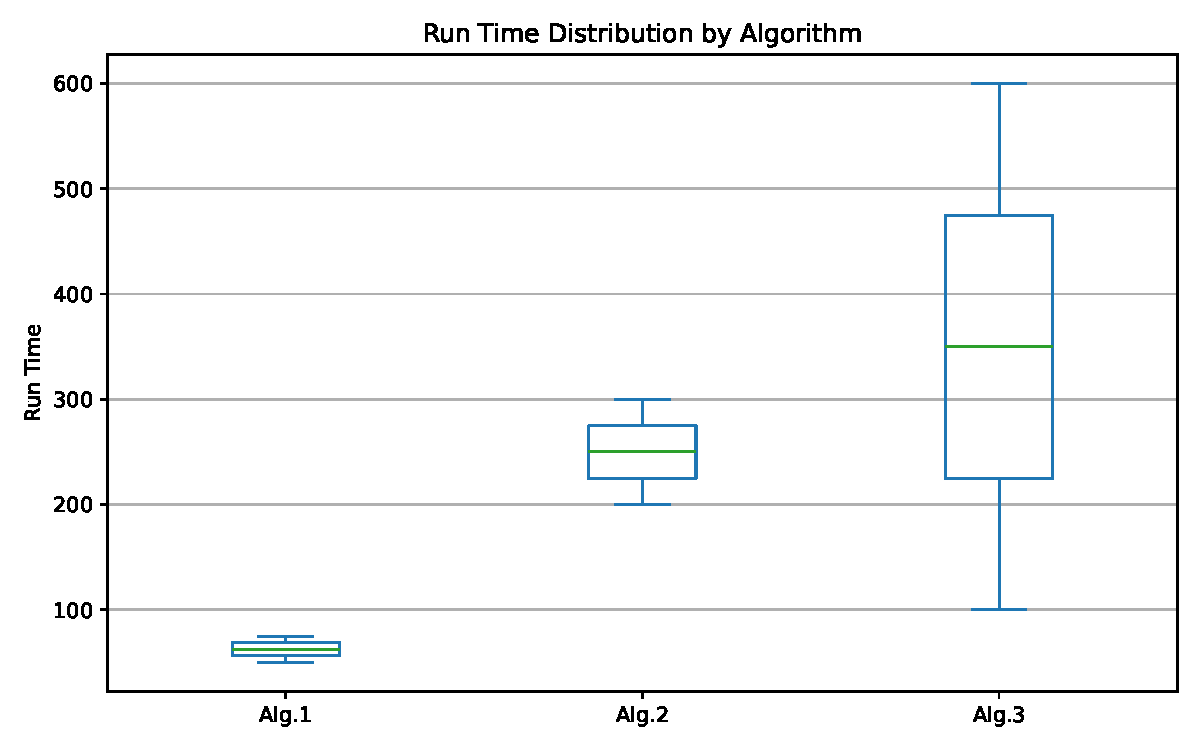
\includegraphics[width=0.8\textwidth]{box_before.pdf} 
		\caption{نمودار جعبه‌ای توزیع زمان اجرای هر الگوریتم}
		\label{fig:box-before}
	\end{figure}
	\textbf{تحلیل:} نمودار جعبه‌ای میزان پراکندگی (وُاریانس) زمان اجرای هر الگوریتم را نشان می‌دهد. جعبه الگوریتم $3$ بسیار کشیده است که نشان می‌دهد زمان اجرای آن نوسان بالایی داشته و بازه گسترده‌ای را در بر می‌گیرد. در مقابل، جعبه الگوریتم $1$ بسیار فشرده است که نشانگر ثبات و تغییرات اندک این الگوریتم در مواجهه با افزایش اندازه داده ورودی است.
	
	\subsection{به‌روزرسانی داده‌ها (افزودن داده $700$ کیلوبایت)}
	طبق بند (ب) صورت سوال، ردیف جدیدی برای داده‌های با حجم $700$ کیلوبایت (با زمان‌های $80$، $320$ و $700$ برای الگوریتم‌های $1$ تا $3$) مستقیماً به فایل اکسل اضافه شد. به دلیل اینکه کد پایتون به صورت کاملاً پویا\footnote{\lr{Dynamic}} نوشته شده است، بدون هیچ تغییری در سورس کد، برنامه مجدداً اجرا گردید و نمودارها به صورت خودکار با داده‌های جدید به‌روزرسانی شدند.
	
	نمودارهای به‌روزشده در شکل‌های \ref{fig:line-after} تا \ref{fig:box-after} آورده شده‌اند.
	
	\begin{figure}[H]
		\centering
		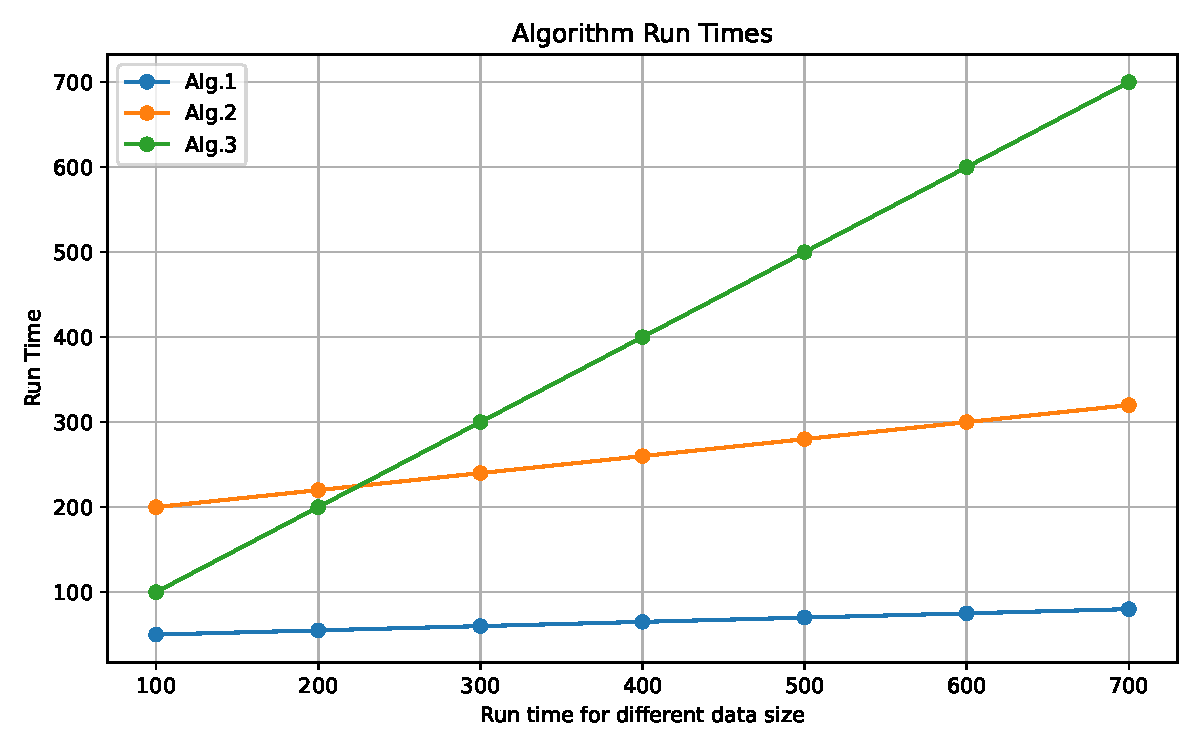
\includegraphics[width=0.8\textwidth]{line_after.pdf}
		\caption{نمودار خطی زمان اجرا پس از افزودن داده $700$ کیلوبایت}
		\label{fig:line-after}
	\end{figure}
	
	\begin{figure}[H]
		\centering
		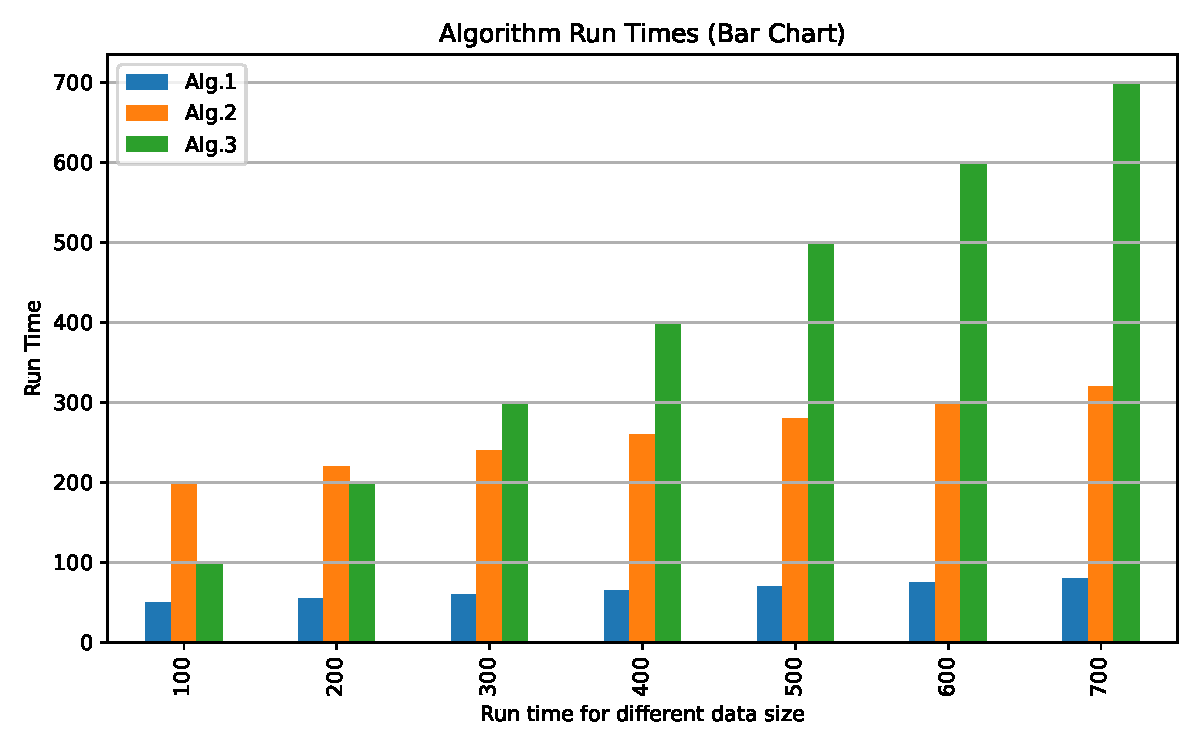
\includegraphics[width=0.8\textwidth]{bar_after.pdf} 
		\caption{نمودار میله‌ای زمان اجرا پس از افزودن داده $700$ کیلوبایت}
		\label{fig:bar-after}
	\end{figure}
	
	\begin{figure}[H]
		\centering
		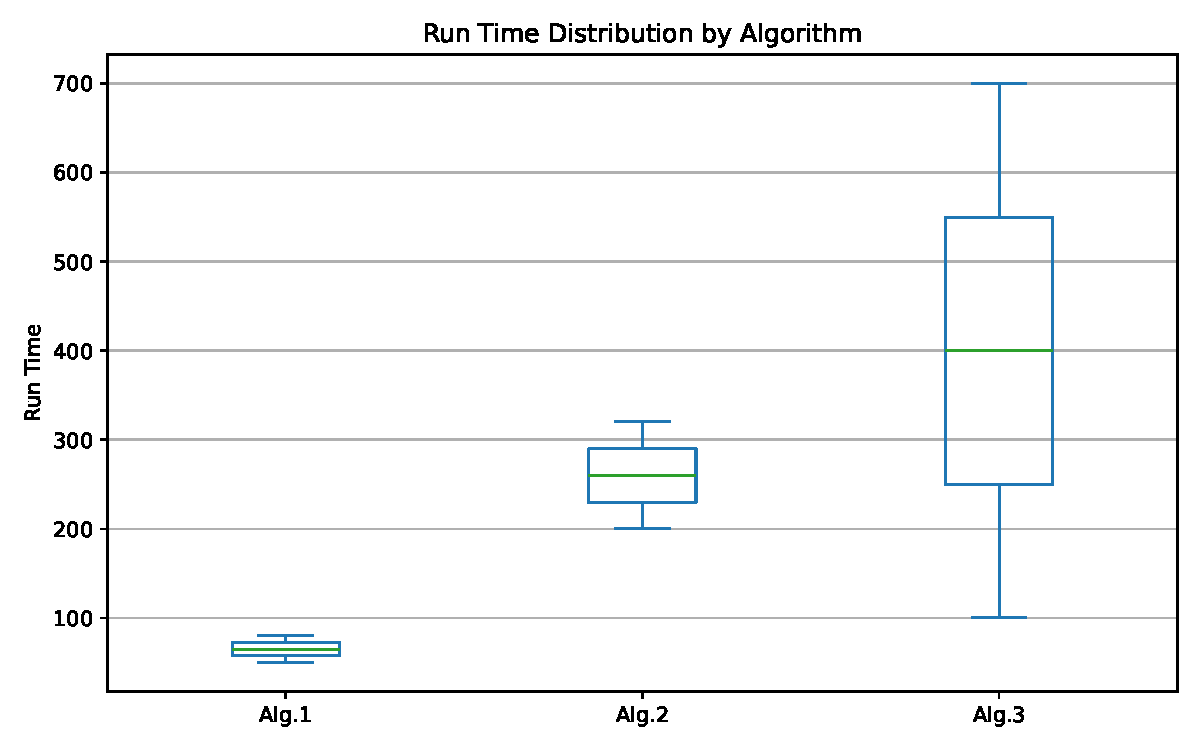
\includegraphics[width=0.8\textwidth]{box_after.pdf} 
		\caption{نمودار جعبه‌ای توزیع زمان اجرا پس از افزودن داده $700$ کیلوبایت}
		\label{fig:box-after}
	\end{figure}
	
	\textbf{تحلیل پس از افزودن داده‌ها:} با اضافه شدن داده $700$ کیلوبایت، محور $X$ در نمودارها به‌طور خودکار گسترش یافته است. نکته قابل توجه، ادامه روند صعودی شدید الگوریتم $3$ تا مقدار $700$ است که باعث شده در نمودار جعبه‌ای، کشیدگی جعبه این الگوریتم نسبت به قبل بیشتر هم بشود. الگوریتم $1$ همچنان با زمان اجرای $80$، بهترین و پایدارترین عملکرد را در حجم داده‌های بزرگ به نمایش می‌گذارد.
	
	\subsection{محاسبه میانگین زمان اجرای الگوریتم $2$}
	در بخش (ج) خواسته شده بود که میانگین زمان اجرای الگوریتم $2$ تنها برای داده‌های با حجم $100$ الی $600$ کیلوبایت محاسبه شود. کد این بخش با استفاده از فیلتر کردن ایندکس‌های دیتافریم بین $100$ و $600$ پیاده‌سازی شد.
	
	در \figurename~\ref{fig:avg-code} کد مربوط به محاسبه میانگین آورده شده است.
	
	\begin{figure}[H]
		\centering
		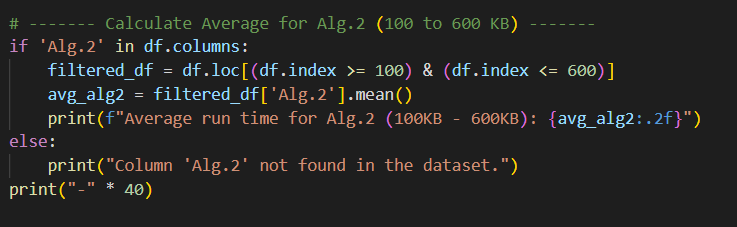
\includegraphics[width=0.95\textwidth]{avg_code.png} 
		\caption{کد پایتون برای محاسبه میانگین الگوریتم $2$ در بازه مشخص}
		\label{fig:avg-code}
	\end{figure}
	
	پس از اجرای کد، خروجی چاپ شده در ترمینال مطابق \figurename~\ref{fig:avg-result} به دست آمد.
	
	\begin{figure}[H]
		\centering
		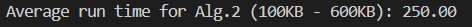
\includegraphics[width=0.7\textwidth]{avg_result.png} 
		\caption{خروجی ترمینال و نمایش مقدار میانگین محاسبه شده}
		\label{fig:avg-result}
	\end{figure}
	
	همان‌طور که در تصویر خروجی مشخص است، سیستم با موفقیت داده‌های ردیف $100$ تا $600$ را فیلتر کرده و داده $700$ کیلوبایتی (در صورت وجود در فایل اکسل) را در این محاسبه دخالت نداده است و مقدار دقیق میانگین چاپ شده است.
	\section{محاسبهٔ انتگرال $f(x) = e^{x^2}$ }
	
	\subsection{صورت مسئله}
	در این بخش، هدف محاسبهٔ انتگرال معین تابع غیرخطی $f(x) = e^{x^2}$ در بازهٔ $[0,1]$ است. این تابع فاقد پادمشتق مقدماتی برحسب توابع ابتدایی است؛ از این رو برای محاسبهٔ انتگرال آن از روش‌های تقریب عددی استفاده می‌شود. روش‌های پیاده‌سازی شده در این بخش شامل موارد زیر هستند:
	\begin{enumerate}
		\item \textbf{قاعدهٔ ذوزنقه:} تقسیم بازه به زیربازه‌های مساوی و تقریب زیر نمودار با استفاده از ذوزنقه‌ها.
		\item \textbf{قاعدهٔ سیمپسون:} تقریب منحنی با استفاده از سهمی‌های عبوری از نقاط میانی هر دو زیربازه (تعداد زیربازه‌ها زوج در نظر گرفته می‌شود).
		\item \textbf{انتگرال‌گیری گاوسی:} استفاده از گره‌ها و وزن‌های بهینه‌سازی‌شده برای دستیابی به بیشترین دقت ممکن با کمترین تعداد ارزیابی تابع.
	\end{enumerate}
	
	\subsection{کد پایتون و پیاده‌سازی}
	پیاده‌سازی این روش‌ها در زبان پایتون با بهره‌گیری از کتابخانه‌های علمی انجام شده است. کد استفاده شده برای این محاسبات به همراه چاپ خروجی مستقیم برای هر روش در \figurename~\ref{fig:integration-code} نمایش داده شده است.
	
	\begin{figure}[H]
		\centering
		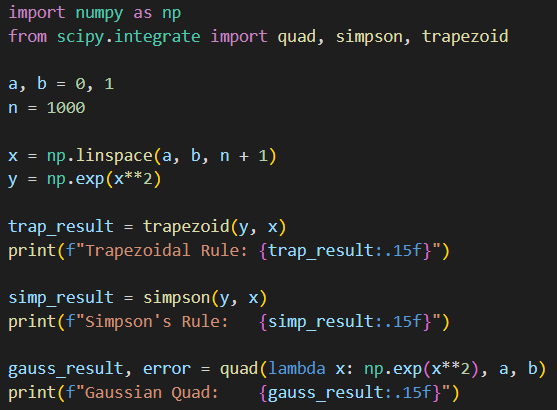
\includegraphics[width=0.95\textwidth]{integration_code.png} 
		\caption{کد پایتون برای محاسبهٔ انتگرال به روش‌های ذوزنقه، سیمپسون و انتگرال‌گیری گاوسی}
		\label{fig:integration-code}
	\end{figure}
	
	\subsection{نتایج و خروجی اجرای برنامه}
	پس از اجرای کد بالا بر روی بازهٔ مشخص‌شده با تعداد زیربازه‌های $1000$ ($n=1000$), نتایج عددی تا $15$ رقم اعشار به دست آمد. خروجی چاپ شده در محیط ترمینال در \figurename~\ref{fig:integration-result} نمایش داده شده است.
	
	\begin{figure}[H]
		\centering
		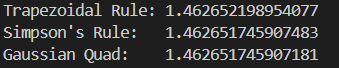
\includegraphics[width=0.95\textwidth]{integration_result.png} 
		\caption{خروجی اجرای کد و مقادیر انتگرال محاسبه شده}
		\label{fig:integration-result}
	\end{figure}
	
	مقادیر استخراج شده از خروجی برنامه به شرح زیر است:
	\begin{itemize}
		\item \textbf{قاعدهٔ ذوزنقه:} $1.462652198954077$
		\item \textbf{قاعدهٔ سیمپسون:} $1.462651745907483$
		\item \textbf{انتگرال‌گیری گاوسی:} $1.462651745907181$
	\end{itemize}
	
	\subsection{تحلیل و مقایسهٔ روش‌ها}
	با بررسی و مقایسهٔ نتایج عددی به دست آمده از این سه روش، نکات زیر قابل تحلیل است:
	\begin{enumerate}
		\item \textbf{خطای روش ذوزنقه:} روش ذوزنقه به دلیل استفاده از تقریب‌های خطی ساده در هر بازه، دارای بیشترین میزان خطا در مقایسه با سایر روش‌ها است. این موضوع خود را در تفاوت ارقام اعشار از مرتبهٔ هفتم به بعد در مقایسه با روش گاوسی نشان می‌دهد.
		\item \textbf{دقت روش سیمپسون:} روش سیمپسون به دلیل استفاده از درون‌یابی درجهٔ دو (سهموی) در هر دو زیربازهٔ متوالی، به طرز چشمگیری دقیق‌تر از روش ذوزنقه است. مشاهده می‌شود که این روش تا $12$ رقم اعشار با نتیجهٔ حاصل از انتگرال‌گیری گاوسی مطابقت دارد.
		\item \textbf{کارایی و قدرت انتگرال‌گیری گاوسی:} روش انتگرال‌گیری گاوسی پیاده‌سازی شده در کتابخانهٔ علمی پایتون، به عنوان مرجع دقیق در نظر گرفته می‌شود. این روش با استفاده از انتخاب هوشمندانهٔ نقاط ارزیابی (گره‌ها) و تخصیص وزن‌های بهینه به آن‌ها، بدون نیاز به افراز بازه به بخش‌های بسیار زیاد، دقیق‌ترین مقدار ممکن را برای انتگرال توابع هموار فرموله می‌کند.
	\end{enumerate}
	\section{دسترسی به کدهای پروژه}
	تمامی کدهای برنامهٔ پایتون، نمودارهای تولیدشده، فایل‌های داده و فایل گزارش این پروژه در یک مخزن عمومی در بستر گیت‌هاب بارگذاری شده و جهت ارزیابی در دسترس است. 
	
	برای مشاهده و بررسی جزئیات کدهای پروژه، می‌توانید به آدرس زیر مراجعه فرمایید:
	\begin{center}
		\url{https://github.com/rahimiparham2001/mathematical-software-projects.git}
	\end{center}
\end{document}
